%! TEX root = ../main.tex

\titre{Le language de requête SQL}

\section{Requêtes SQL}

\subsection{{Bases de données relationnelles}}

Comment organiser et interagir avec des giganstesques quantité de données ? Cette question est à l'origine d'un champ crucial de l'informatique : les \textit{systèmes de gestion de bases de données} (SGBD). Un SGBD est un logiciel dont la charge est précisément de stocker, organiser et accéder à un ensemble de données. Leur fonctionnement est extrêmement complexe, nous nous contenterons d'apprendre à \textit{interagir} avec ces systèmes, par le biais du langage SQL (pour \textit{Structured Query Language}).


Plus précisément, nous nous intéressons au bases de données dites \textit{relationnelles} (BDR). Schématiquement, les bases de données relationnelles sont composées de plusieurs \textit{tables} (sorte d'équivalent des tableaux bidimensionnels d'Excel), et de \textit{relations} entre ces tables. Par exemple, dans la base de données \textsc{Mondial} (voir le site \href{The MONDIAL Database}{https://www.dbis.informatik.uni-goettingen.de/Mondial/}), qui contient pléthore d'informations géographiques et socio-économiques à l'échelle mondiale, on trouve une table \texttt{country} qui contient 6 \textit{attributs}, voir \autoref{tab:country}


\begin{table}[h!]
	\centering
	\begin{tabular}{|cccccc|}
		\hline
		\texttt{Name} & \texttt{Code}$ \star $ & \texttt{Capital} & \texttt{Province} & \texttt{Area}                        & \texttt{Population} \\
		              &                        &                  &                   & Surface du pays en $ \textrm{km}^2 $ &                     \\
		\hline
	\end{tabular}
	\caption{la table \texttt{country} }
	\label{tab:country}
\end{table}

Un attribut est simplement le nom donné à une des colonnes de la table. Un \textit{enregistrement}, ou \textit{entrée}, est une ligne de la table. Par exemple, voici les 3 premiers enregistrements de la table \texttt{country}
\begin{table}[h!]
	\centering
	\begin{tabular}{|cccccc|}
		\hline
		\texttt{Name} & \texttt{Code}$ \star $ & \texttt{Capital} & \texttt{Province} & \texttt{Area} & \texttt{Population} \\ \hline
		Albania       & AL                     & Tirana           & Albania           & 28750         & 281977              \\
		Greece        & GR                     & Athina           & Attixis           & 131940        & 10432481            \\
		Cyprus        & CY                     & Nicosia          & Cyprus            & 9251          & 918100              \\ \hline
	\end{tabular}
	\caption{3 premiers enregistrements de la table \texttt{country} }
	\label{tab:country}
\end{table}

En général, une table contient un grand nombre d'enregistrements et l'utilisateurs connaît uniquement le nom des attributs de la table (il y a trop d'enregistrements pour tous les regarder individuellement).

\subsubsection*{Clefs primaires}
Que veut dire le symbole $ \star $ à côté de l'attrubut \texttt{Code} ? C'est une indication pour signifier que l'attribut \texttt{Code} forme la clef primaire de la table \texttt{country}, c'est-à-dire que chaque enregistrement de la table possède une valeur pour \texttt{Code} distincte (il n'y a pas de doublons). Ainsi, la valeur de \texttt{Code} permet d'identifier \textit{uniquement} un enregistrement de la table ; par exemple GR identifie uniquement la seconde entrée de \texttt{country}.

En général, la clef primaire est constituée d'un seul attribut -- mais ce n'est pas obligatoire. Par exemple, il existe une table \texttt{encompasses}, toujours dans la base de données \textsc{Mondial}, dont la clef primaire est le couple d'attributs \texttt{(Country, Continent)} -- voir \autoref{tab:encompasses}. La table \texttt{encompasses} indique pour chaque pays les continents dans lequel se trouve le pays et la pourcentage de la surface du pays dans chacun de ces coninents. L'attribut \texttt{country} seul n'est pas une clef primaire car il est possible qu'un pays soit à cheval sur plusieurs continents (par exemple la Russie, représentée par un "R" dans la table).


\begin{table}[h!]
	\begin{tabular}{|ccc|}
		\hline
		\texttt{Country}$ \star $                 & \texttt{Continent}$ \star $ & \texttt{Percentage}                                 \\
		Clef étrangère pour \texttt{country.Code} &                             & Pourcentage de la surface du pays dans le continent \\ \hline
		R                                         & Europe                      & 23.15                                               \\
		R                                         & Asia                        & 76.85                                               \\
		RA                                        & South America               & 100                                                 \\
		RB                                        & Africa                      & 100                                                 \\ \hline
	\end{tabular}
	\caption{4 premières entrées de la table \texttt{encompasses}}
	\label{tab:encompasses}
\end{table}
\subsubsection*{Clef étrangère}

Dans la table \texttt{encompasses}, vous aurez peut être remarqué que \texttt{Country} est une "clef étrangère pour \texttt{country.Code}". Qu'est-ce que cela signifie ?

Tout l'intérêt des bases de données relationnelles est de considérer les tables non pas individuellement mais comme un ensemble lié par des relations. Une clef étrangère permet de mettre en correspondance les lignes d'une table avec les lignes d'une autre table, en mettant en relation la clef étrangère de la première avec la clef primaire de la seconde. En l'occurrence, cela signifie simplement qu'un enregistrement de la table \texttt{encompasses} dont l'attribut \texttt{Country} est, par exemple, FR évoque le même pays que l'enregistrement de \texttt{country} dont l'attribut \texttt{Code} est FR.

Cela nous permettra par exemple de créer une grande table rassemblant à la fois les informations de \texttt{Country} et \texttt{Code}, appelée une \textit{jointure}. Une image vallant mille mots, regarder \autoref{fig:jointure}. Une telle table pourra être utile pour par exemple répondre à la question "Quelle est la surface totale d'Europe?".

\begin{figure}[h]
	\begin{center}
		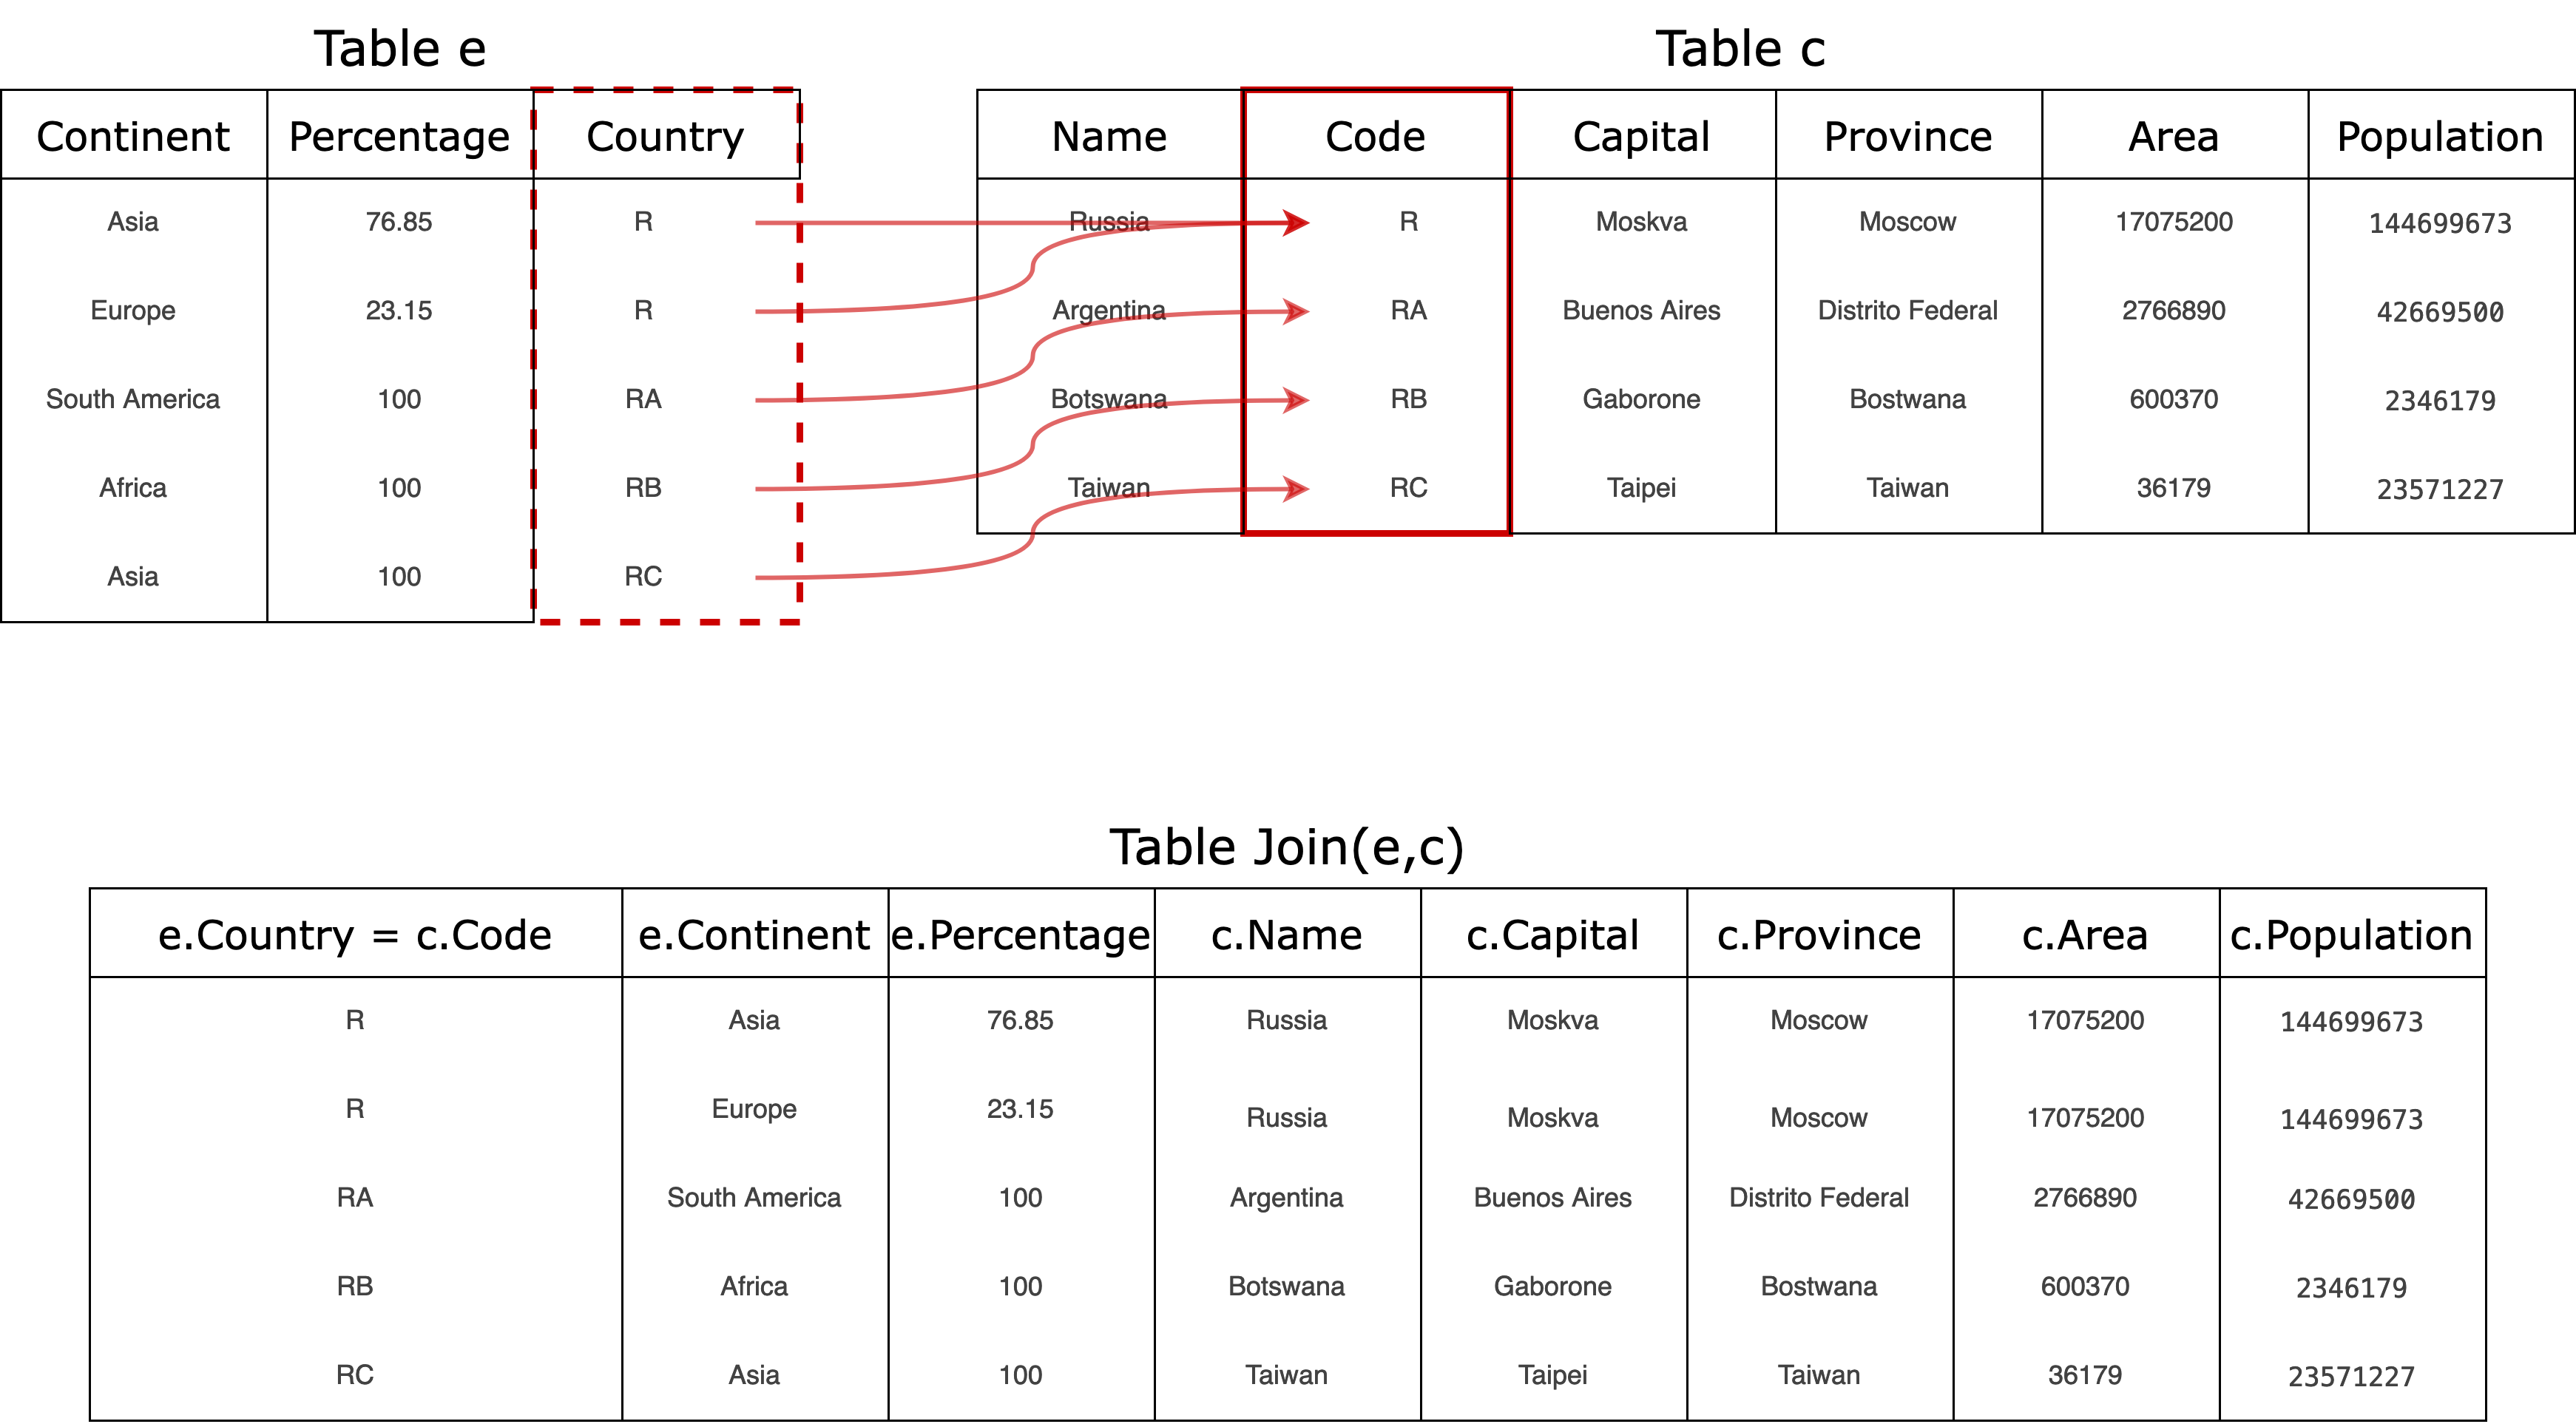
\includegraphics[width=0.95\textwidth]{figures/12/bddr-mondial.png}
	\end{center}
	\caption{Jointure de \texttt{encompasses} et \texttt{country} sur $ \texttt{encompasses.Country} = \texttt{country.Code} $ }
	\label{fig:jointure}
\end{figure}


\subsection{Le language SQL}

Comme mentionné avant, le language SQL permet d'interagir avec le système de base de données : manipuler des tables, extraire des enregistrements, sélectionner certains attributs, faire des jointures, etc. On opte ici par une présentation du language par l'exemple, en augmentant petit à petit le niveau de difficulté.

\subsubsection*{Pour tester ses requêtes en ligne}

Il pourra être utile de tester les requêtes réellement sur la base de données \textsc{Mondial}. Pour cela, suivre les instructions suivantes :
\begin{enumerate}
	\item aller sur la page \href{https://sqliteonline.com/}{https://sqliteonline.com/}.
	\item cliquer sur \texttt{Import} dans la barre d'outils du haut et importer le fichier de base de données que vous pouvez télécharger à l'adresse \href{https://gabriel.belouze/tps/data/bdd-mondial.sql}{https://gabriel.belouze/tps/data/bdd-mondial.sql}, qui crée le sous-ensemble de \textsc{Mondial} avec lequelle on va travailler.
	\item  cliquer sur OK. Vous devriez voir apparaître dans la barre de gauche les tables \texttt{Country}, \texttt{City}, \texttt{Economy}, \texttt{Encompasses}, \texttt{Spoken}.
\end{enumerate}

Ensuite, il suffit d'écrire les requêtes dans l'éditeur de texte et de les tester avec le bouton \texttt{Run}.

\subsubsection{Premiers pas}

Regardons juste l'attribut \texttt{Name} de la table \texttt{country}.

\begin{minted}{sql}
    SELECT Name FROM country;
\end{minted}

Remarquez que les requêtes SQL se terminent par un point virgule. Remarquez également que SQL ne fait pas la différence entre minuscules et majuscules, on aurait tout aussi bien pu écrire

\begin{minted}{sql}
    SeleCt NAMe froM COUNTry;
\end{minted}

Traditionnellement, les mots clefs (ici \mintinline{sql}{SELECT} et \mintinline{sql}{FROM}) sont écrits tout en majuscules.

Regardons les attributs \texttt{Area} et \texttt{Population} de la table \texttt{country}
\begin{minted}{sql}
    SELECT Area, Population FROM Country;
\end{minted}

Remarque : contrairement à \texttt{Python}, les espaces, retours à la ligne et indentations ne sont pas importants en SQL. On aurait tout aussi bien pu écrire
\begin{minted}{sql}
    SELECT
                    Area,
                Population             FROM 

        Country
    ;
\end{minted}

Mais évidemment, une bonne indentation clarifiera la lecture et relecture de vos requêtes.

\quessques Écrire une requête pour obtenir les pays du monde et leurs capitales.
\ssques Écrire une requête pour obtenir toute la table \texttt{country}

\paragraph*{} Lorsque l'on veut récupérer l'intégralité d'une table, il devient pénible de devoir écrire le nom de tous les attributs. SQL permet de mettre le symbole \mintinline{sql}{*} à la place. Ainsi, votre dernière requête aurait pu s'écrire

\begin{minted}{sql}
    SELECT * FROM Country;
\end{minted}

\paragraph*{Conditions} La requête suivante répond à la question : quels sont les pays de plus de 100 000 000 habitants ?

\begin{minted}{sql}
    SELECT Name FROM Country WHERE Population > 100000000;
\end{minted}

On peut créer des conditions plus complexes grâce aux opérateurs \mintinline{sql}{OR} et \mintinline{sql}{AND}, par exemple voici une requête pour trouver les petits pays (de surface inférieure à 50 000 $ \textrm{km}^2 $) mais à grande densité de population (plus que 600 habitants par $ \textrm{km}^2 $).

\begin{minted}{sql}
    SELECT Name
        FROM Country
        WHERE Area < 50000 AND Population / Area > 600;
\end{minted}


\paragraph*{Tri du résultat} On peut aussi obtenir la même liste mais triée dans l'ordre croissant

\begin{minted}{sql}
    SELECT Name 
        FROM Country 
        WHERE Population > 100000000 
        ORDER BY Name ASC;
\end{minted}

Ou dans l'ordre décroissant

\begin{minted}{sql}
    SELECT Name 
        FROM Country 
        WHERE Population > 100000000 
        ORDER BY Name DESC;
\end{minted}

\paragraph*{Tronquer le résultat} On peut limiter le nombre de résultat avec la syntaxe \mintinline{sql}{LIMIT n}, où \texttt{n} est un entier. On peut aussi ignorer les \texttt{m} premiers enregistrements du résultat avec la syntaxe \mintinline{sql}{OFFSET m}. Par exemple, la requête suivante trouve les 5 premiers pays (pour l'ordre alphabétique) dont la population dépasse 100M

\begin{minted}{sql}
    SELECT Name
        FROM Country
        WHERE Population > 100000000
        ORDER BY Name ASC
        LIMIT 5;
\end{minted}

et les 3 suivants

\begin{minted}{sql}
    SELECT Name
        FROM Country
        WHERE Population > 100000000
        ORDER BY Name ASC
        LIMIT 3
        OFFSET 5;
\end{minted}

\ques Rédiger une requête pour obtenir
\ssques les 3 pays les plus peuplés du monde, avec leur population correspondante.
\ssques le 4e et 5e pays le moins peuplé du monde.


\subsubsection{Jointures}
Jusque là on n'a pu considérer les tables qu'une par une. Comment faire en SQL l'équivalent de ce qui est représenté \autoref{fig:jointure} ? Voici par exemple une requête pour obtenir les pays d'Europe

\begin{minted}{sql}
    SELECT country.Name
        FROM country JOIN encompasses ON country.Code = encompasses.Country
        WHERE encompasses.Continent = "Europe";
\end{minted}

La partie \mintinline{sql}{country JOIN encompasses ON country.Code = encompasses.Country} crée une table similaire à celle représentée \autoref{fig:jointure}, c'est-à-dire dont les attributs sont

\begin{table}[h!]
	\centering
	\begin{tabular}{|ccccc|}
		\hline
		\texttt{country.Name}       & \texttt{country.Code}        & \texttt{country.Capital}       & \texttt{country.Province}       & \texttt{country.Area} \\
		\texttt{country.Population} & \texttt{encompasses.Country} & \texttt{encompasses.Continent} & \texttt{encompasses.Percentage} &                       \\
		\hline
	\end{tabular}
\end{table}

et dans laquelle pour chaque enregistrement $ country.Code $ et $ encompasses.Country $ sont égaux.

Pour éviter de devoir écrire le nom complet de la table d'origine, on peut fournir des noms plus courts avec le mot clef \mintinline{sql}{AS}. Ainsi la requête précédente aurait pu s'écrire

\begin{minted}{sql}
    SELECT c.Name
        FROM country AS c JOIN encompasses AS e ON c.Code = e.Country
        WHERE e.Continent = "Europe";
\end{minted}

\ques Rédiger une requête pour obtenir
\ssques les pays du continent américain qui comptent moins de 10 habitants par $ \textrm{km}^2 $.
\ssques les capitales européennes situées à une latitude supérieure à $ 60^{\circ} $.
\ssques les pays ayant plus de 1 000 000 $ \textrm{km}^2 $ dans l'Asie, triés par surface de territoire asiatique décroissante. Donner également la valeur de cette surface de territoire asiatique.

\subsubsection{Fonctions d'agrégation}

SQL donne également accès à des fonctions qui réalisent des calculs sur l'ensemble d'une table, les fonctions d'agrégation. \autoref{tab:important-agregation-func} rassemble les plus importantes de ces fonctions (et celles qqui sont au programme).

\begin{figure}[h!]
	\centering
	\begin{tabular}{|ll|}
		\hline
		\mintinline{sql}{COUNT()} & nombre d'enregistrements      \\
		\mintinline{sql}{MAX()}   & valeur maximale d'un attribut \\
		\mintinline{sql}{MIN()}   & valeur minimale d'un attribut \\
		\mintinline{sql}{SUM()}   & somme d'un attribut           \\
		\mintinline{sql}{AVG()}   & moyenne d'un attribut         \\
		\hline
	\end{tabular}
	\caption{Fonctions d'agrégation}
	\label{tab:important-agregation-func}
\end{figure}

Ainsi la requête suivante calcule le nombre de pays en Asie

\begin{minted}{sql}
    SELECT COUNT(Country) FROM Encompasses WHERE Continent="Asia";
\end{minted}

Puisqu'ici on compte juste le nombre de lignes, la colonne que l'on donne à l'intérieur de \mintinline{sql}{COUNT(...)} n'importe pas. Il est donc plus élégant d'écrire

\begin{minted}{sql}
    SELECT COUNT(*) FROM Encompasses WHERE Continent="Asia";
\end{minted}

\ques Rédiger une requête pour obtenir
\ssques la surface totale du continent \texttt{Africa}.
\ssques la population mondiale.
\ssques la population moyenne par pays.
\ssques le nombre de pays de plus de 1 000 000 de $ \textrm{km}^2 $

% \subsubsection{Groupements}
%
%
% La base de données \texttt{Mondial} possède également une table \texttt{spoken}, décrite \autoref{tab:spoken}.
%
% \begin{table}
% 	\centering
%
% 	\begin{tabular}{|ccc|}
% 		\hline
% 		\texttt{Country}$ \star $                 & \texttt{Language}$ \star $ & \texttt{Percentage}                                      \\
% 		Clef étrangère pour \texttt{country.Code} &                            & Pourcentage de la population du pays qui parle la langue \\
% 		\hline
% 	\end{tabular}
% 	\caption la table \texttt{spoken}
% 	\label{tab:spoken}
% \end{table}
%

% \newpage
